\section{Введение}
\subsection{Фаззинг}
Фаззинг (fuzzing) - это автоматизированный метод тестирования программного обеспечения, при котором система генерирует случайные или модифицированные входные данные с целью выявления ошибок, уязвимостей и сбоев в работе программы \cite{Kuliamin}. Данный метод тестирования позволяет находить ситуации, которые могут привести к неожиданному поведению программы или быть использованы злоумышленниками для эксплуатации уязвимостей \cite{Manes}.

Фаззинг стал ключевым инструментом обеспечения безопасности программного обеспечения благодаря высокой степени автоматизации и способности находить редкие и критические ошибки \cite{Manes}. Он играет важную роль в современной практике разработки ПО, особенно в условиях роста зависимости от open-source решений \cite{Boehme}.

Крупные компании (например, Google, Microsoft, Samsung) активно применяют фаззинг для поиска уязвимостей в своих продуктах. Таким обращом, фаззинг уже стал промышленным стандартом обеспечения качества и безопасности ПО \cite{Boehme}.

Существует несколько подходов к классификации фаззеров \cite{Kuliamin}\cite{Boehme}:
\begin{itemize}
	\item \textbf{По уровню доступа}:
	\begin{itemize}
		\item Черный ящик: фаззинг без использования информации о внутреннем состоянии программы.
		\item Серый ящик: использование частичной информации о покрытии кода.
		\item Белый яшик: полное знание структуры программы, часто используется символьное исполнение.
	\end{itemize}
	\item \textbf{По типу генерации входных данных}
	\begin{itemize}
		\item Мутационные фаззеры - изменяют существующие примеры входных данных.
		\item Генеративные фаззеры - создают новые данные <<по шаблону>>.
	\end{itemize}
	\item \textbf{По анализу выполнения:}
	\begin{itemize}
		\item На основе покрытия кода (coverage-guided fuzzing).
		\item Символьное исполнение (symbolic execution).
		\item Тайнт-анализ (Dynamic Taint Analysis, DTA) - метод динамического анализа программного обеспечения, предназначенный для отслеживания распространения <<помеченных>> данных в ходе выполнения программы. Позволяет, например, отследить утечку конфиденциальных данных \cite{Kuliamin}.
	\end{itemize}
\end{itemize}

Современные фаззеры используют различные техники для увеличения эффективности тестирования \cite{Kuliamin}\cite{Boehme}:
\begin{itemize}
	\item \textbf{Фаззинг с обратной связью по покрытию (Coverage-guided fuzzing)} - наиболее распространенная техника, при которой фаззер отслеживает участки кода, достигаемые текущим корпусом, и генерирует новые входные данные, которые открывают новые ветви выполнения.
	\item \textbf{Гибридный фаззинг}  комбинирует фаззинг с динамической символьной интерпретацией (DSE), позволяя целенаправленно исследовать сложные ветви логики.
	\item \textbf{Эволюционные алгоритмы} используются для оптимизации процесса мутации входных данных
	\item \textbf{Модельный фаззинг (Model-based fuzzing)} полагается на формальные спецификации или прототипы формата для генерации корректных, но потенциально опасных входных данных.
\end{itemize}

Несмотря на широкое применение, фаззинг-тестирование имеет ряд ограничений \cite{Kuliamin}\cite{Boehme}:
\begin{enumerate}
	\item Труднорешаемые логические условия препятствуют продвижению фаззера.
	\item Ошибки зависят от состояния системы, что делает их сложно воспроизводимыми.
	\item Недерминированное поведение параллельных потоков усложняет анализ.
	\item Злоумышленники и разработчики ПО могут использовать обфускацию кода, маскировку ошибок и обнаружение режима фаззинга для снижения его эффективности.
\end{enumerate}

Таким образом, фаззинг остаётся одним из наиболее перспективных и действенных методов обеспечения надёжности и безопасности программного обеспечения в условиях растущего числа угроз и сложности современных систем.

\subsection{libFuzzer}
Тестовые сценарии разработаны с ипользованием библиотеки libFuzzer. \textbf{libFuzzer} - это встраиваемый фаззер с обратной связью по покрытию и поддержкой эволюционных алгоритмов мутации входных данных. Он разработан как часть проекта LLVM \cite{Libfuzzer}.

libFuzzer использует следующие техники и стратегии фаззинга:
\begin{itemize}
	\item \textbf{Фаззинг с обратной связью по покрытию}.
	\item \textbf{Эволюционные алгортмы} для мутации входных данных.
	\item \textbf{Поддержка словарей}: позволяет задавать характерные последовательности для формата входных данных.
	\item \textbf{Параллелизм}: поддерживает запуск нескольких процессов фаззинга с общим корпусом.
\end{itemize}

Ключевые компоненты libFuzzer:
\begin{itemize}
	\item \textbf{fuzz target}: точка входа для фаззера (целевая функция). Это пользовательская функция \FunName{LLVMFuzzerTestOneInput}, которая принимает массив байтов и передает его тестируемому коду. Эта функция должна быть детерминированной, для воспроизводимости тестов.
	\item \textbf{Корпус (Corpus)}: набор входных данных для фаззинга.
	\item \textbf{SanitizerCoverage}: инструмент LLVM, обеспечивающий сбор информации о покрытии кода. Он позволяет определить фаззеру, какие части кода были выполнены.
	\item \textbf{Механизмы мутации}: встроенные стратегии изменения входных данных, например, вставка, удаление, замена, скрещивание и другие.
	\item \textbf{Санитайзеры}: поддерживает интеграцию с AddressSanitizer, UBSan, MSan и LeakSanitizer.
\end{itemize}
\begin{figure}[htbp]
	\centering % Центрирование
	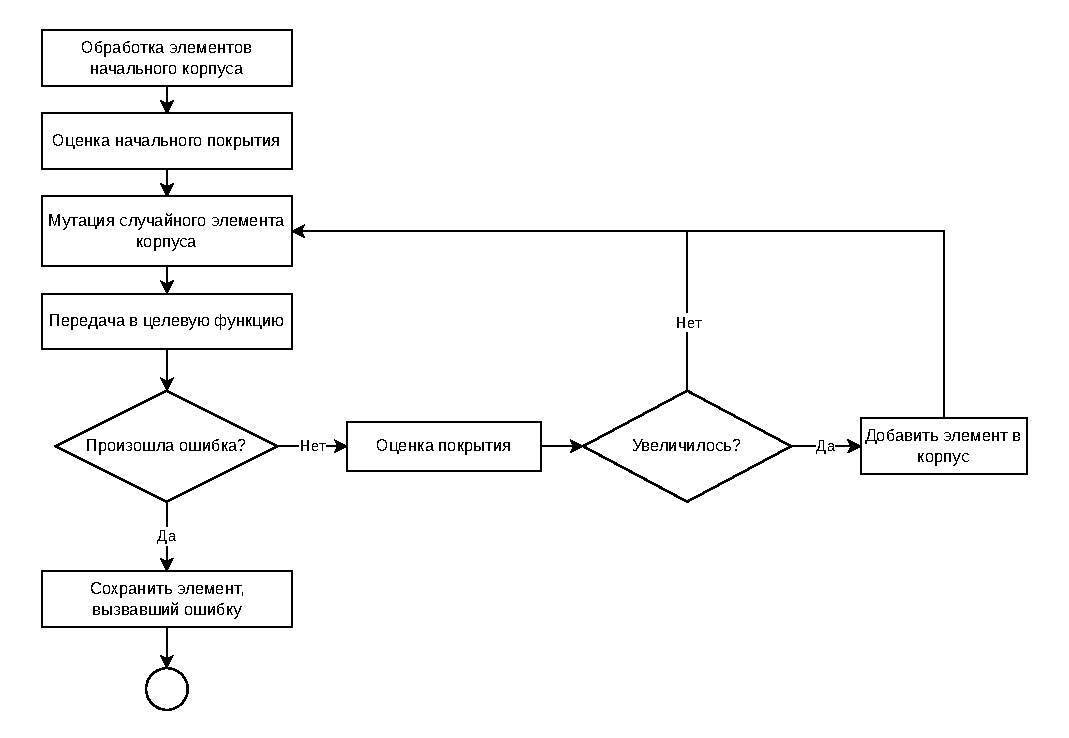
\includegraphics[width=0.8\textwidth]{Piclibfuzz.pdf} % Путь к файлу
	\caption{Общая схема работы фаззера с использованием libFuzzer.} % Подпись
	\label{intro:libfuzz} % Метка для ссылок
\end{figure}
Работа фаззера (см. рисунок \ref{intro:libfuzz}) начинается с инициализации корпуса, после чего запускается основной цикл: выбирается элемент из корпуса, мутирует, передается в целевую функцию и оценивается результат. В случае успешного увеличения покрытия или обнаружения ошибки (завершение с ошибкой, утечка памяти, таймаут) состояние сохраняется. Процесс продолжается бесконечно или прерывается в случае обнаружения ошибки. В последнем случае тест, вызвавший ошибку, сохраняется отдельно для последующего точечного воспроизведения.

\subsection{UEFI-окружение и драйверы}
\textbf{Unified Extensible Firmware Interface (UEFI)} - это интерфейс между операционной системой и прошивкой платформы (firmware), заменяющий устаревший BIOS.  Интерфейс обеспечивает взаимодействие между аппаратными средствами платформы и программным обеспечением, таким как загрузчик операционной системы. UEFI является ключевым компонентом современной архитектуры загрузки и инициализации аппаратных платформ, предоставляя расширенные возможности по сравнению с традиционной BIOS: поддержка модульности, драйверов, файловых систем, SecureBoot, сетевые функции и другие механизмы \cite{UEFISpec}.

В контексте UEFI драйвер предоставляет собой модуль, реализующий поддержку конкретного оборудования или логического устройства через один или несколько стандартизированных протоколов. Драйверы могут загружаться как вместе с прошивкой, так и с внешнего носителя по запросу приложения и работать в UEFI-среде до передачи упрвления ОС.

\begin{figure}[htbp]
	\centering % Центрирование
	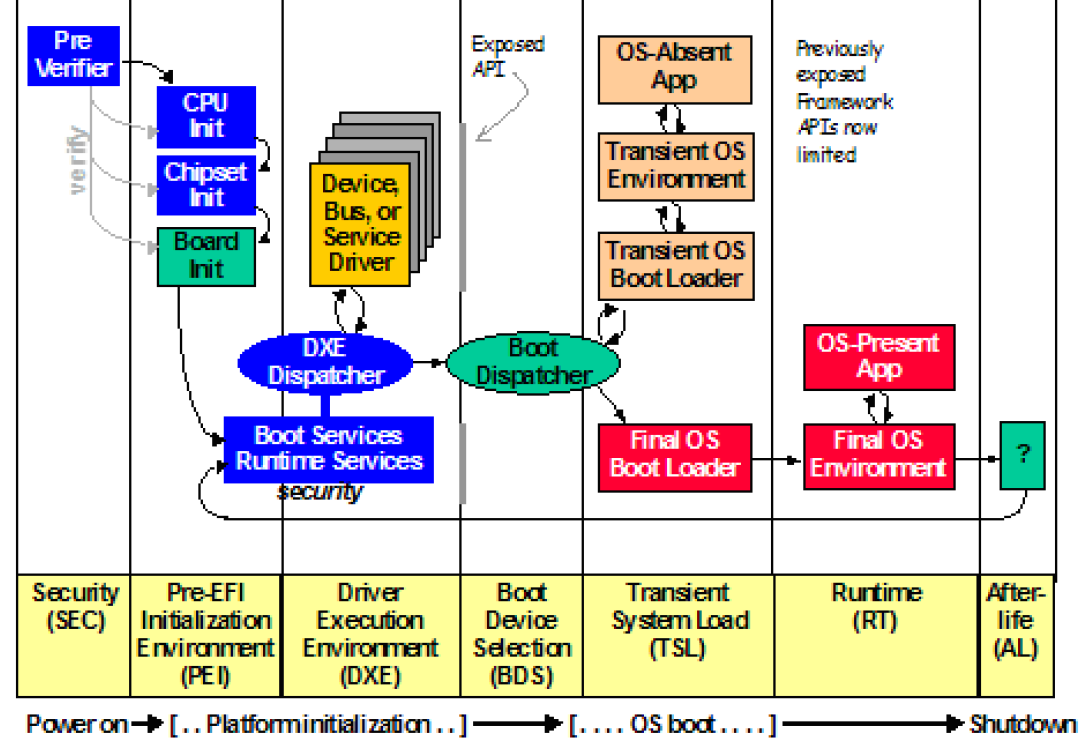
\includegraphics[width=0.5\textwidth]{piphases.png} % Путь к файлу
	\caption{Фазы инициализации платформы \cite{UEFIPI}.} % Подпись
	\label{intro:piphases} % Метка для ссылок
\end{figure}
Спецификация \cite{UEFIPI} описывает архитектуру инициализации платформы, разбитую на несколько фаз (см. рисунок \ref{intro:piphases}), каждая из которых имеет свои особенности и допустимые типы драйверов:
\begin{itemize}
	\item \textbf{PEI Drivers, PEIM}. Выполняются в фазе PEI. Отвечают за минимальную инициализацию оборудования, используют ограниченный набор сервисов: PEI Services и PEI Private Interfaces.
	\item \textbf{DXE Drivers}. Основные драйверы, запускающиеся в фазе DXE (Driver Execution Enviroment), обеспечивают поддержку UEFI Boot Services и Runtime Services. Драйверы файловых систем обычно относятся к этому типу.
	\item \textbf{SMM Drivers}. Драйверы, которые работают в режиме SMM (System Managment Mode) и предназначены для обработки аппаратных прерываний вне контекста ОС (например, драйверы термоконтроля).
	\item \textbf{UEFI Application Driver}. Некоторые UEFI-приложения могут запустить по требованию драйвер с внешнего носителя.
\end{itemize} 

В контексте UEFI протоколы предоставляют собой стандартизированные интерфейсы, через которые компоненты среды могут предоставлять и использовать определенные функциональные возможности. Протоколы реализуются как структуры данных (таблицы), содержащие указатели на функции, различные поля с данными и указатели на другие протоколы. Протоколы идентифицируются уникальным GUID (Globally Unique Identifier), что позволяет найти все реализации конкретного протокола в среде.

 Драйвер файловой системы должен реализовывать протокол \VarName{EFI\_FILE\_PROTOCOL}. Данный протокол предоставляет унифицированный интерфейс для работы с файловой системой: открытие файлов, чтение/запись, удаление, получение информации о файлах, чтение содержимого каталогов. В спецификации определены две версии:
 \begin{itemize}
 	\item \VarName{EFI\_FILE\_PROTOCOL\_REVISION} описывает только синхронные операции.
 	\item \VarName{EFI\_FILE\_PROTOCOL\_REVISION2} описывает синхронные и асинхронные операции.
 \end{itemize}
 
В данной работе для тестирования драйверов применяется базовое UEFI-окружение в пользовательском пространстве, предоставляемое проектом \GitName{Acidanthera/OpenCorePkg} \cite{OpenCorePkg}. Ключевые преимущества этого подхода перед тестированием в реальной среде UEFI:
\begin{itemize}
	\item Полный доступ к функционалу libFuzzer и LLVM Sanitizer's:
	\begin{itemize}
		\item Запуск нескольких процессов фаззинга  одновременно.
		\item Информативное описание результатов тестирования.
		\item Простой доступ к тестам, вызывающим ошибки.
	\end{itemize}
	\item Отладка стандартными средствами GDB.
	\item Изолированное тестирование конкретного драйвера.
\end{itemize}
 
 Тестируются драйверы FAT, ext4 (предоставляемые проектом \GitName{Acidanthera/audk} \cite{Audk}) и EFI NTFS, предоставляемый проектом \cite{OpenCorePkg}.  